\documentclass[12font]{article}
\title{\textbf{ Many-Body Entanglement and Correlation Matrix}}
\author{Chen-Chih Wang  }
\date{\textit{Department of physics, National Tsing Hua University, Hsinchu 30013, Taiwan} \\ (Dated: \today)}
\usepackage[margin=2cm]{geometry}
%\usepackage[fleqn]{amsmath}
%\usepackage{CJK,amsmath}
\usepackage{amsfonts,amssymb}
\usepackage{fancyhdr}
%\pagestyle{fancy}
\usepackage{textcomp}
\usepackage{graphicx}
\usepackage{float}
\usepackage{color}
\usepackage{tikz}
\usepackage{multicol}
\usepackage{threeparttable}
\usepackage{amsthm}
\usepackage{mathtools}
\usepackage{hyperref}
\urlstyle{same}
\usepackage{caption}
\usepackage{subcaption}
\usepackage{dsfont}
\usepackage{comment}
\newtheorem{theorem}{Theorem}[section]
\theoremstyle{definition}
\newtheorem{definition}{Definition}[section]
\newtheorem{lemma}[theorem]{Lemma}
\newtheorem{corollary}{Corollary}[theorem]
\newtheorem{proposition}[theorem]{Proposition}

\numberwithin{equation}{section}

\newcommand{\vac}{\mrm{vac}}
\newcommand{\Bra}[1]{\left\langle #1 \right|}
\newcommand{\Ket}[1]{\left| #1 \right\rangle}
\newcommand{\bra}[1]{\langle #1 |}
\newcommand{\ket}[1]{| #1 \rangle}
\newcommand{\angleLr}[1]{\left\langle #1 \right\rangle}
\newcommand{\anglelr}[1]{\langle #1 \rangle}
\newcommand{\braket}[2]{\langle #1 | #2 \rangle}
\newcommand{\Bbraket}[2]{\left\langle #1 \right|\left. #2 \right\rangle}
\newcommand{\dif}[1]{\frac{\mathrm{d}}{\mathrm{d}#1}}
\newcommand{\diff}[2]{\frac{\mathrm{d}#1}{\mathrm{d}#2}}
\newcommand{\gd}{\boldsymbol{\nabla}}
\newcommand{\dive}{\boldsymbol{\nabla}\cdot}
\newcommand{\curl}{\boldsymbol{\nabla}\times}
\newcommand{\llr}[1]{(  #1  )}
\newcommand{\llrm}[1]{[  #1  ]}
\newcommand{\llrg}[1]{\{  #1  \}}
\newcommand{\lr}[1]{\left(  #1  \right)}
\newcommand{\lrm}[1]{\left[  #1  \right]}
\newcommand{\lrg}[1]{\left\{  #1  \right\}}
\newcommand{\abs}[1]{\left|  #1  \right|}
\newcommand{\de}{\partial}
\newcommand{\pdif}[1]{\frac{\partial}{\partial#1}}
\newcommand{\pdiff}[2]{\frac{\partial#1}{\partial#2}}
\newcommand{\mrm}[1]{\mathrm{#1}}
\newcommand{\bo}[1]{\mathbf{#1}}
\newcommand{\bog}[1]{\boldsymbol{#1}}
\newcommand{\vint}[3]{\int_{#1}#2\cdot\mathrm{d}\mathbf{#3}}
\newcommand{\voint}[3]{\oint_{#1}#2\cdot\mathrm{d}\mathbf{#3}}
\newcommand{\Vint}{\int\mrm{d}^3\bo{r}'}
\newcommand{\rr}{\mathbf{r} - \mathbf{r}'}
\newcommand{\arr}{\left|\mathbf{r} - \mathbf{r}'\right|}
\newcommand{\nx}{\hat{\bo{n}}_1}
\newcommand{\ny}{\hat{\bo{n}}_2}
\newcommand{\alert}[1]{{\color{red}#1}}
\newcommand{\alertV}[1]{{\color{violet}#1}}
\newcommand{\Tr}{\mrm{Tr}}
\newcommand{\tr}{\mrm{tr}}
\newcommand{\norm}[1]{\left\lVert#1\right\rVert}
\newcommand{\im}{\mrm{i}}

\newcommand{\kbond}[2]{\sigma_{#1}^{\alpha_{{#1}{#2}}}\sigma_{#2}^{\alpha_{{#1}{#2}}}}
\newcommand{\kbondSpe}[3]{\sigma_{#1}^{#3}\sigma_{#2}^{#3}}

\newcommand{\wordfig}[2]{\begin{minipage}[h]{#1 cm}
	\vspace{0pt}
	\includegraphics[width=\textwidth]{#2}
   \end{minipage}}

\begin{document}
\maketitle
%\fontsize{12pt}{18pt}\selectfont
\begin{abstract}
  Here we overview the \emph{correlation matrix} technique for computing the entanglement entropy. After build a general formalism for the technique, we then try to investigate the entanglement of a parton mean-field theory.
\end{abstract}

\tableofcontents

\section{Unification of Second-Quantization Notation}
In the mathematical frame work of the second quantization, we first build the Fock space for many-particles, and then define the creation and annihilation operators -- $c$ and $c^\dagger$ -- to generate those Fock basis vectors. Here, we can define a new notation to unify every operators to make the calculation more neat. In this note, we only focus on fermionic operators. Nevertheless, the notation we are going to discuss can be used to bosonic cases as well, just by some simple modifications.

In general, a fermion localized at the position $i$ possessing quantum numbers $\sigma$ (angular momentum, band, spin, valley, colour, etc.) can be represented by $c_{i\sigma}$ and $c_{i\sigma}^\dagger$, standing for annihilation and creation respectively. Here we treat Hermition conjugation $\dagger$ as a new quantum number, I call it \emph{particle-hole quantum number}, and define a new operator to unify the creation and the annihilation operators in the following way,
\begin{equation}\label{uni-def.e}
  c_{i\sigma\aleph} = \begin{cases}
                        c_{i\sigma} &;\quad \aleph=0 \\
                        c_{i\sigma}^\dagger &;\quad \aleph=1
                      \end{cases}
\end{equation}
where the quantum number $\aleph=0\vee 1$ stands for annihilation and creation. For notational convenience for later discussions, we define $\overline{\aleph}$ as the \emph{flipping} of Hermition conjugation, i.e. $\overline{0} = 1$ and $\overline{1}=0$. Therefore,
\begin{equation}\label{flipping-bar.e}
  c_{i\sigma\aleph}^\dagger = c_{i\sigma\overline{\aleph}}
\end{equation}
For fermions, we have the relation as \emph{definitions} for fermion statistics,
\[
\begin{aligned}
& \llrg{c_{i\sigma}, c_{j\sigma'}^\dagger} = \delta_{ij}\delta_{\sigma\sigma'} \\
& \llrg{c_{i\sigma}, c_{j\sigma'}} = 0
\end{aligned}
\]
Using our notation, these two conditions can be unified to a single equation\footnote{For bosons, the commutation conditions can be unifies as
\[
\llrm{b_{i\sigma\aleph},b_{j\sigma'\aleph'}} = \delta_{ij}\delta_{\sigma\sigma'}\epsilon_{\aleph\aleph'}
\]
where $\epsilon_{ij}$ is the antisymmetric tensor, $\epsilon_{01}=-\epsilon_{10} = 1$ and $\epsilon_{00} = 0 = \epsilon_{11}$}
\begin{equation}\label{commutation-def.e}
  \llrg{c_{i\sigma\aleph},c_{j\sigma'\aleph'}} = \delta_{ij}\delta_{\sigma\sigma'}\delta_{\aleph\overline{\aleph'}}
\end{equation}

Traditionally, we define the \emph{vacuum state} $\ket{0}$ in the way that
\[
c_{i\sigma}\ket{0} = 0
\]
Applying a creation operator on such a state generate a \emph{single occupied} state, denoted by
\[
\ket{i\sigma} = c^\dagger_{i\sigma}\ket{0}
\]
and 
\[
c^\dagger_{i\sigma}\ket{i\sigma} = 0
\]
So the occupied state can be seen as the \emph{vacuum state} of the hole to some extend. Using our notation, The basis with different particle numbers in the Fock space can be unified in the way that they are all in the same space but just with different particle-hole quantum numbers,
\[
\ket{\llrg{i},\llrg{\sigma},\llrg{\aleph}}
\]
such that, take single particle case for example,
\[
\begin{aligned}
& c_{i\sigma\aleph}\ket{i\sigma\aleph} = 0 \\
& c_{i\sigma\overline{\aleph}}\ket{i\sigma\aleph} = \ket{i\sigma\overline{\aleph}} 
\end{aligned}
\]
and
\[
\ket{\cdots , i_1\sigma_1\aleph_1, \cdots, i_2\sigma_2\aleph_2,\cdots} = (-1)^{\aleph_1\aleph_2}\ket{\cdots, i_2\sigma_2\aleph_2, \cdots, i_1\sigma_1\aleph_1,\cdots}
\]
because the exchange with a \emph{vacuum} won't cause any sign changing. In these examples, we have shown that in the particle-hole quantum number notation framework, the creation or annihilation are just changing of the particle-hole quantum numbers\footnote{Such a picture is no longer valid for bosons because a single state can be occupied by more than one bosons.}. The vacuum state is just a many-particle state with all particle-hole quantum numbers $\aleph=0$.

\section{Bogoliubov Transform of Normal Fermions}
In the particle-hole quantum number language, the Bogoliubov transform is nothing but a generalized basis transformation. A Bogoliubove transform from a normal fermion $c$ to a normal fermion $f$ can be expressed as
\[
f_{i\sigma\aleph} = \sum_{j\sigma'\aleph'}\phi^{j\sigma'\aleph'}_{i\sigma\aleph}c_{j\sigma'\aleph'}
\]
Where $\phi^{j\sigma'\aleph'}_{i\sigma\aleph} \in \mathbb{C}$ are coefficients. To make the new fermion $f$ to be a normal fermion, the coefficients $\phi$ can't be chosen arbitrary. There are several conditions that $\phi$ has to obey. 

First and the simplest requirement is to make sure 
\[
f_{i\sigma\aleph}^\dagger = f_{i\sigma\overline{\aleph}} = \sum_{j\sigma'\aleph'}\phi^{j\sigma'\aleph'}_{i\sigma\overline{\aleph}}c_{j\sigma'\aleph'}
\]
So
\[
\sum_{j\sigma'\aleph'}\phi^{j\sigma'\aleph'}_{i\sigma\overline{\aleph}}c_{j\sigma'\aleph'} = f_{i\sigma\aleph}^\dagger = \sum_{j\sigma'\aleph'}\lrm{\phi^{j\sigma'\aleph'}_{i\sigma\aleph}}^* c_{j\sigma'\overline{\aleph'}} = \sum_{j\sigma'\aleph'}\lrm{\phi^{j\sigma'\overline{\aleph'}}_{i\sigma\aleph}}^* c_{j\sigma'\aleph'} 
\]
Therefore, we have
\begin{equation}\label{hermitian-change.e}
   \lrm{\phi^{j\sigma'\aleph'}_{i\sigma\aleph}}^*= \phi^{j\sigma'\overline{\aleph'}}_{i\sigma\overline{\aleph}}
\end{equation}
In the particle-hole quantum number language, the normal transform is nothing but a special case of the generalized Bogoliubov transform, where $\phi^{j\sigma'\aleph'}_{i\sigma\aleph} = \phi^{j\sigma'}_{i\sigma}\delta_{\aleph\aleph'}$. To make sure $f$ is a normal fermion, it is required to satisfy the anticommutation relation (\ref{commutation-def.e}). So, 
\begin{align*}
    \llrg{f_{i\sigma\aleph},f_{j\sigma'\aleph'}} &= \sum_{kk'}\sum_{\eta\eta'}\sum_{\gimel\gimel'} \phi^{k\eta\gimel}_{i\sigma\aleph} \phi^{k'\eta'\gimel'}_{j\sigma'\aleph'} \llrg{ c_{k\eta\gimel}, c_{k'\eta'\gimel'} }\\ 
    &= \sum_{kk'}\sum_{\eta\eta'}\sum_{\gimel\gimel'} \phi^{k\eta\gimel}_{i\sigma\aleph} \phi^{k'\eta'\gimel'}_{j\sigma'\aleph'} \delta_{kk'} \delta_{\eta\eta'}\delta_{\gimel\overline{\gimel'}} \\
    &= \sum_{k}\sum_{\eta}\sum_{\gimel} \phi^{k\eta\gimel}_{i\sigma\aleph} \phi^{k\eta\overline{\gimel}}_{j\sigma'\aleph'} \\
    &= \sum_{k}\sum_{\eta}\sum_{\gimel} \phi^{k\eta\gimel}_{i\sigma\aleph} \lrm{\phi^{k\eta\gimel}_{j\sigma'\overline{\aleph'}}}^*\\
    &=\delta_{ij}\delta_{\sigma\sigma'}\delta_{\aleph\overline{\aleph'}}
\end{align*}
So we have
\begin{equation}\label{unitary.e}
  \sum_{k}\sum_{\eta}\sum_{\gimel} \phi^{k\eta\gimel}_{i\sigma\aleph} \lrm{\phi^{k\eta\gimel}_{j\sigma'\aleph'}}^* =\delta_{ij}\delta_{\sigma\sigma'}\delta_{\aleph\aleph'}
\end{equation}
which shows the unitary feature of the coefficients $\phi$. If the Bololiubov transform is invertible, then we need another condition
\begin{equation}\label{unitary-true.e}
  \sum_{k}\sum_{\eta}\sum_{\gimel} \phi_{k\eta\gimel}^{i\sigma\aleph} \lrm{\phi_{k\eta\gimel}^{j\sigma'\aleph'}}^* =\delta_{ij}\delta_{\sigma\sigma'}\delta_{\aleph\aleph'}
\end{equation}
The physical meaning of a \emph{invertible Bogoliubov transform} is that \emph{the number of independent $c$-modes is the same as the number of independent $f$-modes}. In a mathematical way, that is equivalent to say that a matrix $V$ with $V^\dagger V=\mathds{1}$ doesn't mean $V V^\dagger = \mathds{1}$. The latter one holds only if $V$ is invertible, and vice versa.

\section{Reduced Density Matrix and Correlation Matrix}
For a fermion system, any local operator at the site $i$ can be represented by the following basis operators,
\[
c_{i\sigma} \quad,\quad c_{i\sigma}^\dagger \quad,\quad c^\dagger_{i\sigma}c_{i\sigma'} \quad,\quad c_{i\sigma}c^\dagger_{i\sigma'}
\]
with different quantum numbers $\sigma$ and $\sigma'$. Following the method and notations used in Ref.\cite{toeplitz}, any local operators defined inside the region $A$ can be expanded by these basis,
\[
\mathcal{O}_A = \sum_{n}C_n\bigotimes_{i\in A}\mathcal{O}_i^{(n)}
\]
each $\mathcal{O}_i^{(n)}$ is one of the basis operators listed above. The coefficients $C_n\in\mathbb{C}$ are coefficients to be determined. If the local operator $\mathcal{O}_A^{(n)}$ we are considering is the reduced density matrix of the region $A$, then the coefficients are nothing but the expectation values of those basis operators. That is,
\begin{equation}\label{rho_A-raw-form.e}
  \rho_A = \sum_{n}\angleLr{\bigotimes_{i\in A}\mathcal{O}_i^{(n)}}\bigotimes_{i\in A}\mathcal{O}_i^{(n)}
\end{equation}

Consider a free-fermion model haing the following general form,
\[
H = \sum_{ij}\sum_{\sigma\sigma'}\lr{t_{ij}^{\sigma\sigma'} c_{i\sigma}^\dagger c_{j\sigma'} + \Delta_{ij}^{\sigma\sigma'}c_{i\sigma}c_{j\sigma'}} + \mrm{H.c.}
\]
the correlation function of fermions in the ground state can be decomposed into product of two-point correlation functions by Wick's theorem. In light of this, we can do a \emph{local} Bogoliubov transformation, as what the author of Ref.\cite{toeplitz} did, 
\[
d_{i\sigma} = \sum_{j\in A}\sum_{\sigma'}\lr{u^{j\sigma'}_{i\sigma}c_{j\sigma'} + v^{j\sigma'}_{i\sigma}c^\dagger_{j\sigma'}}
\]
where $u,v\in\mathbb{C}$, such that
\[
\anglelr{d^\dagger_{i\sigma} d_{j\sigma'}} = \lambda_{i\sigma}\delta_{ij}\delta_{\sigma\sigma'} \quad,\text{and}\quad \anglelr{d_{i\sigma}d_{j\sigma'}} = 0
\]
We will see this is doable later. Because $d$-fermions are superpositions of $c$-fermions, we can also use Wick's theorem to decompose the multi-point correlation functions of $d$-fermion operators into product of two-point functions. Plus the fact that the coefficients in the expression \ref{rho_A-raw-form.e} are nothing but multi-point correlation functions of $d$-fermion operators, those coefficients can be decomposed into two-point correlation functions. In the end of the day, the reduced density matrix can be factorized in the following form, as shown in the equation (19) of Ref.\cite{toeplitz},
\begin{equation}\label{rho_A-factorize.e}
\rho_A = \bigotimes_{i\in A}\bigotimes_{\sigma}\lrm{\anglelr{d^\dagger_{i\sigma}d_{i\sigma}} d^\dagger_{i\sigma}d_{i\sigma} + \anglelr{d_{i\sigma}d^\dagger_{i\sigma}}d_{i\sigma}d^\dagger_{i\sigma}} = \bigotimes_{i\in A}\bigotimes_{\sigma}\lrm{\lambda_{i\sigma}d^\dagger_{i\sigma}d_{i\sigma} + \llr{1-\lambda_{i\sigma}}d_{i\sigma}d^\dagger_{i\sigma}}
\end{equation}
With this, it is easy to prove that the entanglement entropy is
\[
S_A = -\Tr_A\rho_A\ln\rho_A = -\sum_{i\sigma}\lrm{\lambda_{i\sigma}\ln\lambda_{i\sigma} + \llr{1-\lambda_{i\sigma}}\ln\llr{1-\lambda_{i\sigma}}}
\]
In light of this, if we define a matrix as
\begin{equation}\label{b-corrmatrix-def.e}
  G^{(d)}_{i\sigma,j\sigma'} \equiv \anglelr{d^\dagger_{i\sigma}d_{j\sigma'}} \quad;\quad i,j\in A
\end{equation}
and of course this matrix is already diagonal by our definition of $d$-fermions, then the entanglement entropy can be expressed as
\begin{equation}\label{ee-matrixexpression-1.e}
  S_A = -\tr\lrm{G^{(d)}\ln G^{(d)} + \llr{\mathrm{1} - G^{(d)}}\ln\llr{\mathrm{1}-G^{(d)}}}
\end{equation}
Here we have demonstrated an important conclusion that the entanglement entropy of a free-fermion system can be directly calculated by $G^{(d)}$, dubbed the \emph{correlation matrix} of $d$-fermions. In the next section, we are going to discuss how to get the entanglement entropy from \emph{general} correlation matrices.

\section{Particle-Hole Quantum Number Notation and Correlation Matrix}
We can generalize the correlation matrix (\ref{b-corrmatrix-def.e}) using the particle-hole quantum number notation in the following way,
\begin{equation}\label{correlation-general-def-b.e}
  \mathcal{G}^{(d)}_{i\sigma\aleph,j\sigma'\aleph'} \equiv \anglelr{  d_{i\sigma\aleph}d_{j\sigma'\overline{\aleph'}} } \quad;\quad i,j\in A
\end{equation}
In this way, the correlation matrix contains both $\lambda$ and $(1-\lambda)$ at the same time, so the entanglement entropy is 
\begin{equation}\label{ee-general-b.e}
  S_A = -\tr\lrm{\mathcal{G}^{(d)}\ln\mathcal{G}^{(d)}}
\end{equation}
Formulas (\ref{ee-matrixexpression-1.e}) and (\ref{ee-general-b.e}) tell us that if there exist matrices $U$ and $\mathcal{G}^{(c)}$ such that
\[
\mathcal{G}^{(c)} = U\mathcal{G}^{(d)}U^{-1}
\]
then the entanglement entropy can also be obtained by such a matrix. So our goal is to define the correlation matrix for the original $c$-fermions
\begin{equation}\label{correlation-general-c-def.e}
  \mathcal{G}^{(c)}_{i\sigma\aleph,j\sigma'\aleph'} \equiv \anglelr{  c_{i\sigma\aleph}c_{j\sigma'\overline{\aleph'}} } \quad;\quad i,j\in A
\end{equation}
and see if there exist a matrix $U$ such that $\mathcal{G}^{(c)}$ is equivalent to $\mathcal{G}^{(d)}$. If so, then we can calculate the correlation matrix $\mathcal{G}^{(c)}$ and then diagonalize it to get the entanglement entropy directly. The reason we need to think about this is that most of time there is no simple way to find the Bogoliubov transform to get the perfect $d$-fermions at the first place. But diagonalization is easy to do via numerical methods and the correlation function of $c$-fermions can also be calculated analytically. So the correlation matrix $\mathcal{G}^{(c)}$ is the only hope for this method to be used practically. 

By definition, $d$-fermion is the Bogoliubov transform of $c$-fermion, so again
\[
d_{i\sigma\aleph} = \sum_{j\in A}\sum_{\sigma'\aleph'}\phi^{j\sigma'\aleph'}_{i\sigma\aleph}c_{j\sigma'\aleph'} \quad;\quad i\in A
\]
where the coefficients $\phi$ satisfy the following two conditions
\[
\lrm{\phi^{j\sigma'\aleph'}_{i\sigma\aleph}}^*= \phi^{j\sigma'\overline{\aleph'}}_{i\sigma\overline{\aleph}} 
\quad ,\quad 
\sum_{k\in A}\sum_{\eta}\sum_{\gimel} \phi^{k\eta\gimel}_{i\sigma\aleph} \lrm{\phi^{k\eta\gimel}_{j\sigma'\aleph'}}^* =\delta_{ij}\delta_{\sigma\sigma'}\delta_{\aleph\aleph'} = \sum_{k\in A}\sum_{\eta}\sum_{\gimel} \phi_{k\eta\gimel}^{i\sigma\aleph} \lrm{\phi_{k\eta\gimel}^{j\sigma'\aleph'}}^*
\]
We have to keep in mind that every transformation we are talking about here is entirely inside region $A$. Substitute the Bogoliubov transform into the correlation matrix of $b$-fermion,
\begin{align*}
  \mathcal{G}^{(b)}_{i\sigma\aleph,j\sigma'\aleph'} &= 
  \anglelr{ d_{i\sigma\aleph}d_{j\sigma'\overline{\aleph'}} } \\
  &= \sum_{kk'\in A}\sum_{\eta\eta'}\sum_{\gimel\gimel'} \phi_{i\sigma\aleph}^{k\eta\gimel} \phi_{i\sigma'\overline{\aleph'}}^{k'\eta'\gimel'} \anglelr{c_{k\eta\gimel}c_{k'\eta'\gimel'}} \\
  &=
  \sum_{kk'\in A}\sum_{\eta\eta'}\sum_{\gimel\gimel'} \phi_{i\sigma\aleph}^{k\eta\gimel} \lrm{\phi_{i\sigma'\aleph'}^{k'\eta'\overline{\gimel'}}}^* \anglelr{c_{k\eta\gimel}c_{k'\eta'\gimel'}} \\
  &= 
  \sum_{kk'\in A}\sum_{\eta\eta'}\sum_{\gimel\gimel'} \phi_{i\sigma\aleph}^{k\eta\gimel} \lrm{\phi_{i\sigma'\aleph'}^{k'\eta'\gimel'}}^* \anglelr{c_{k\eta\gimel}c_{k'\eta'\overline{\gimel'}}} \\
  &=
  \sum_{kk'\in A}\sum_{\eta\eta'}\sum_{\gimel\gimel'} \phi_{i\sigma\aleph}^{k\eta\gimel}
  \lrm{\phi_{i\sigma'\aleph'}^{k'\eta'\gimel'}}^* \mathcal{G}^{(c)}_{k\eta\gimel,k'\eta'\gimel'}
\end{align*}
If define a matrix $U$ with elements
\[
[U]_{i\sigma\aleph,j\sigma'\aleph'} = \phi_{i\sigma\aleph}^{j\sigma'\aleph'}
\]
then the relation between $\mathcal{G}^{(b)}$ and $\mathcal{G}^{(c)}$ can be written as
\[
\mathcal{G}^{(b)} = U\mathcal{G}^{(c)}U^\dagger
\]
Thanks for the properties (\ref{unitary.e}) and (\ref{unitary-true.e}), we know that $U$ is unitary,
\[
UU^\dagger = U^\dagger U = \mathds{1}
\]
Therefore, the two correlation matrices $\mathcal{G}^{(b)}$ and $\mathcal{G}^{(c)}$ are equivalent related by the matrix $U$ with matrix elements the coefficients of the Bogoliubov transform.

So, in conclusion, the entanglement entropy of a free-fermion system is
\begin{equation}\label{ee-correlation-final}
  S_A = -\tr\lrm{\mathcal{G}^{(c)}\ln\mathcal{G}^{(c)}}
\end{equation}

\section{Majorana Fermions}
Due to $\gamma^\dagger = \gamma$ for Majorana fermions, the particle-hole quantum number no longer exists. So the method developed in previous sections cannot be used directly.

Consider a set $\Lambda$ of lattices sites as the whole system, and at every site $i\in\Lambda$ we define Majorana fermion operators $\gamma_{i\sigma}$ with different quantum numbers $\sigma$ satisfying $\gamma_{i\sigma}^\dagger = \gamma_{i\sigma}$ for all of them. The dimension of the Hilbert space of the whole system is $\dim\mathcal{H}_\Lambda = 2^{N_{\sigma}\abs{\Lambda}/2}$, where $N_{\sigma}$ is the total amount of the quantum numbers and $\abs{\Lambda}$ is the number of lattice sites in $\Lambda$, because each Majorana fermion carries only half of the dimension. Therefore, the system is well defined if and only if $N_{\sigma}\times\abs{\Lambda}$ is an even number. There are two possibilities. The first one is that $N_{\sigma}$ is even. If so, then $N_{\sigma}\times\abs{\Lambda}$ is always even, and the system is always well defined no matter how many sites inside $\Lambda$. On the other hand, the second case is that $N_{\sigma}$ is odd. In this case, the number of $\abs{\Lambda}$ is important.
\subsection{Even Number of Quantum Numbers}
If $N_{\sigma}$ is even, then the system as well as the subsystems are always well defined regardless of the number of lattice sites. Now, our task is to define the particle-hole quantum number and a usable correlation matrix for Majorana fermions. 

A direct way to define the particle-hole quantum number is to divide the original quantum numbers $\sigma$ into to parts and then assign the one part to $\aleph=0$ and the other part to $\aleph=1$. For example, if the Majorana fermions have spin-1/2 quantum numbers $\uparrow$ and $\downarrow$, then we can assign $\uparrow$ to be $\aleph = 0$ and $\downarrow$ to $\aleph=1$. In such a way, we will naturally have $\gamma_{i\tilde{\sigma}\aleph}$ derived from the original $\gamma_{i\sigma}$ where $\tilde{\sigma}\times\aleph = \sigma$. 

The commutation relation for Majorana fermions is
\[
\llrg{\gamma_{i\sigma},\gamma_{j\sigma'}} = 2\delta_{ij}\delta_{\sigma\sigma'}
\]
Similarly, for particle-hole quantum number notation,
\begin{equation}\label{comm-maj-def.e}
\llrg{\gamma_{i\sigma\aleph},\gamma_{j\sigma'\aleph'}} = 2\delta_{ij}\delta_{\sigma\sigma'}\delta_{\aleph\aleph'}
\end{equation}

As for the correlation matrix, the definition for Majorana fermions will also be a little bit different from the normal fermion cases. A good definition of the Majorana correlation matrix is
\begin{equation}\label{corr-majorana-def.e}
  \Gamma^{(\gamma)}_{i\sigma\aleph,j\sigma'\aleph'} \equiv \anglelr{\gamma_{i\sigma\aleph}\gamma_{j\sigma\aleph'}}
\end{equation}
so that $\Gamma^{(\gamma)}$ is Hermitian.

A normal fermion $f$ can also be composed by Majorana fermion $\gamma$ through Bogoliubov transform. Now we are going to investigate the conditions the Bogoliubov coefficients has to fulfill, just like equations (\ref{hermitian-change.e}) to (\ref{unitary-true.e}). The Bogoliubov transform from a Majorana fermion to a normal fermion is of the form
\[
f_{i\sigma\aleph} = \frac{1}{\sqrt{2}}\sum_{j\sigma'\aleph'} \breve{\varphi}_{i\sigma\aleph}^{j\sigma'\aleph'}\gamma_{j\sigma'\aleph'}
\]
where $\breve{\varphi}\in\mathbb{C}$, and the symbol ˘ on top of $\breve{\varphi}$ stands for the transformation from Majorana to normal fermions. Because $f_{i\sigma\aleph}^\dagger = f_{i\sigma\overline{\aleph}}$ and $\gamma_{i\sigma\aleph}^\dagger = \gamma_{i\sigma\aleph}$, we have
\[
\frac{1}{\sqrt{2}}\sum_{j\sigma'\aleph'} \breve{\varphi}_{i\sigma\overline{\aleph}}^{j\sigma'\aleph'}\gamma_{j\sigma'\aleph'} = f_{i\sigma\overline{\aleph}} 
= f_{i\sigma\aleph}^\dagger
= \frac{1}{\sqrt{2}}\sum_{j\sigma'\aleph'} \lrm{\breve{\varphi}_{i\sigma\aleph}^{j\sigma'\aleph'}}^*\gamma_{j\sigma'\aleph'}
\]
Thus
\begin{equation}\label{hermitian-change-Maj.e}
\lrm{\breve{\varphi}_{i\sigma\aleph}^{j\sigma'\aleph'}}^* = \breve{\varphi}_{i\sigma\overline{\aleph}}^{j\sigma'\aleph'}
\end{equation}
On the other hand, the commutation relation gives another condition,
\begin{align*}
    \llrg{f_{i\sigma\aleph},f_{j\sigma'\aleph'}} 
    &= \frac{1}{2}\sum_{kk'}\sum_{\eta\eta'}\sum_{\gimel\gimel'} \breve{\varphi}^{k\eta\gimel}_{i\sigma\aleph} \breve{\varphi}^{k'\eta'\gimel'}_{j\sigma'\aleph'} \llrg{ \gamma_{k\eta\gimel}, \gamma_{k'\eta'\gimel'} }\\ 
    &= \sum_{kk'}\sum_{\eta\eta'}\sum_{\gimel\gimel'} \breve{\varphi}^{k\eta\gimel}_{i\sigma\aleph} \breve{\varphi}^{k'\eta'\gimel'}_{j\sigma'\aleph'} \delta_{kk'} \delta_{\eta\eta'}\delta_{\gimel\gimel'} \\
    &= \sum_{k}\sum_{\eta}\sum_{\gimel} \breve{\varphi}^{k\eta\gimel}_{i\sigma\aleph} \breve{\varphi}^{k\eta\gimel}_{j\sigma'\aleph'} \\
    &= \sum_{k}\sum_{\eta}\sum_{\gimel} \breve{\varphi}^{k\eta\gimel}_{i\sigma\aleph} \lrm{\breve{\varphi}^{k\eta\gimel}_{j\sigma'\overline{\aleph'}}}^*\\
    &=\delta_{ij}\delta_{\sigma\sigma'}\delta_{\aleph\overline{\aleph'}}
\end{align*}
So, we have
\begin{equation}\label{unitary-Maj.e}
  \sum_{k}\sum_{\eta}\sum_{\gimel} \breve{\varphi}^{k\eta\gimel}_{i\sigma\aleph} \lrm{\breve{\varphi}^{k\eta\gimel}_{j\sigma'\aleph'}}^*\\
    =\delta_{ij}\delta_{\sigma\sigma'}\delta_{\aleph\aleph'}
\end{equation}
For the same reason, if the Bogoliubov transform is invertible, then we should also require
\begin{equation}\label{unitary-ture-Maj.e}
  \sum_{k}\sum_{\eta}\sum_{\gimel} \breve{\varphi}_{k\eta\gimel}^{i\sigma\aleph} \lrm{\breve{\varphi}_{k\eta\gimel}^{j\sigma'\aleph'}}^*\\
    =\delta_{ij}\delta_{\sigma\sigma'}\delta_{\aleph\aleph'}
\end{equation}

Following the same pattern, we now examine if the correlation matrices $\Gamma^{(\gamma)}$ and $\mathcal{G}^{(d)}$ are equivalent. So, define the Bogoliubov transform inside the region $A$,
\[
d_{i\sigma\aleph} = \frac{1}{\sqrt{2}}\sum_{j\in A}\sum_{\sigma'\aleph'} \breve{\varphi}^{j\sigma'\aleph'}_{i\sigma\aleph}\gamma_{j\sigma'\aleph'} \quad;\quad i\in A
\]
then
\begin{align*}
  \mathcal{G}^{(b)}_{i\sigma\aleph,j\sigma'\aleph'} 
  &= 
  \anglelr{ d_{i\sigma\aleph}d_{j\sigma'\overline{\aleph'}} } \\
  &= \frac{1}{2}\sum_{kk'\in A}\sum_{\eta\eta'}\sum_{\gimel\gimel'} \breve{\varphi}_{i\sigma\aleph}^{k\eta\gimel} \breve{\varphi}_{i\sigma'\overline{\aleph'}}^{k'\eta'\gimel'} \anglelr{\gamma_{k\eta\gimel}\gamma_{k'\eta'\gimel'}} \\
  &=
  \sum_{kk'\in A}\sum_{\eta\eta'}\sum_{\gimel\gimel'} \breve{\varphi}_{i\sigma\aleph}^{k\eta\gimel}
  \lrm{\breve{\varphi}_{i\sigma'\aleph'}^{k'\eta'\gimel'}}^* \frac{1}{2}\Gamma^{(\gamma)}_{k\eta\gimel,k'\eta'\gimel'}
\end{align*}
Because, as shown by (\ref{unitary-Maj.e}) and (\ref{unitary-ture-Maj.e}), the transformation $\breve{\varphi}$ is unitary. So the above derivation shows that the correlation matrices $\frac{1}{2}\Gamma^{(\gamma)}$ and $\mathcal{G}^{(b)}$ are equivalent. So, we can make the same conclusion as before that the entanglement entropy can be computed by diagonalizing the Majorana correlation matrix,
\[
S_A = -\tr\lrm{\frac{\Gamma^{(\gamma)}}{2}\ln \lr{\frac{\Gamma^{(\gamma)}}{2}}} = -\frac{1}{2}\tr\lrm{\Gamma^{(\gamma)}\ln\Gamma^{(\gamma)}} + \frac{\ln 2}{2}\tr\Gamma^{(\gamma)}
\]
For the last term, because every diagonal entry of a Majoarana correlation matrix is nothing but unity, we have $\tr\Gamma^{(\gamma)} = N_{\sigma} N^A$, where $N^A$ is the number of sites in the region $A$. So eventually we have
\[
    S_A = -\frac{1}{2}\tr\lrm{\Gamma^{(\gamma)}\ln\Gamma^{(\gamma)}} + \frac{1}{2}N_{\sigma}N^A\ln 2
\]
From such a formula, we can see that the particle-hole quantum number is not important at all and can be absorbed back into the physical index to form the original physical index. By end of the day, we have
\begin{equation}\label{ee-corr-Maj.e}
  S_A = -\frac{1}{2}\tr\lrm{\tilde{\Gamma}^{(\gamma)}\ln\tilde{\Gamma}^{(\gamma)}} + \frac{1}{2}N_{\sigma}N^A\ln 2
\end{equation}
where
\begin{equation}\label{original-correlation.e}
  \tilde{\Gamma}^{(\gamma)}_{i\sigma,j\sigma'} \equiv \anglelr{\gamma_{i\sigma}\gamma_{j\sigma'}}
\end{equation}

\subsection{Odd Number of Quantum Numbers}
Suppose there are $2N$ sites in the region $A$, then we can separate and sort these $2N$ lattice sites into $\alpha$ and $\beta$ sublattices, where $\alpha\cap\beta=\varnothing$ and $\alpha\cup\beta=A$, with $N$ lattice sites in each sublattice. After that, we assign $\alpha$ to the particle-hole quantum number $\aleph=0$ and $\beta$ to $\aleph=1$. After defining the particle-hole quantum number, the discussions about the Bogoliubov transform, correlation matrices, and the entanglement entropy are exactly the same as the previous section. So, following the same pattern, one will get the same conclusion as equation (\ref{ee-corr-Maj.e}) that the entanglement entropy is
\[
S_A = -\frac{1}{2}\tr\lrm{\tilde{\Gamma}^{(\gamma)}\ln\tilde{\Gamma}^{(\gamma)}} + \frac{1}{2}N_{\sigma}N^A\ln 2
\]
where $\tilde{\Gamma}^{(\gamma)}$ is defined in the same way as (\ref{original-correlation.e}).

\section{Fermi-Surfaces and Fermi-Points}
\begin{figure}[H]
  \centering
  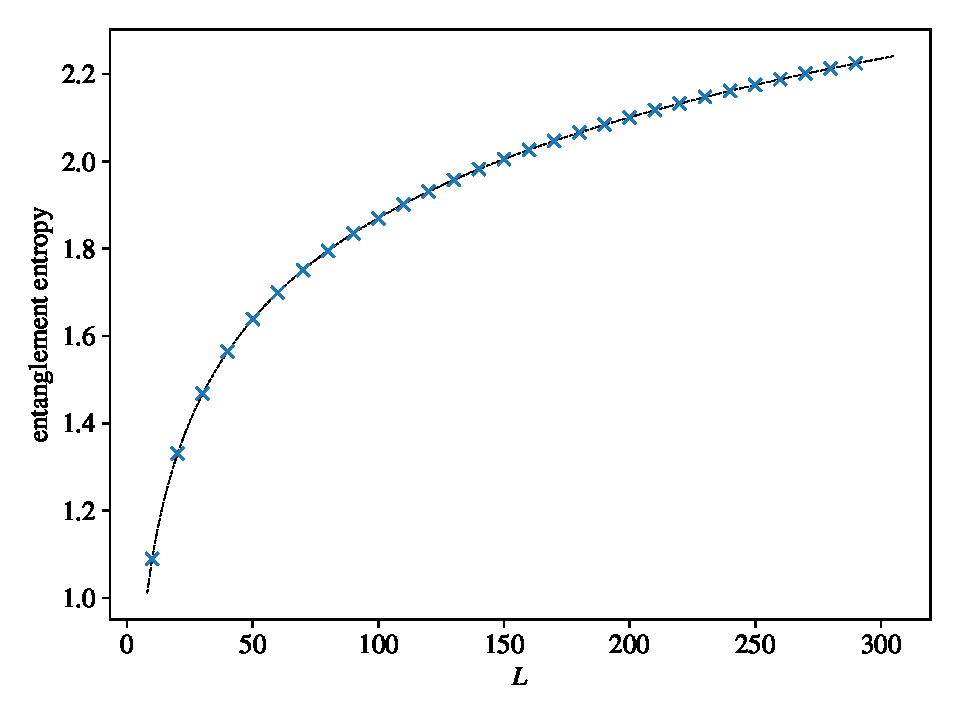
\includegraphics[height=0.15\textheight]{1D_free_fermion}
  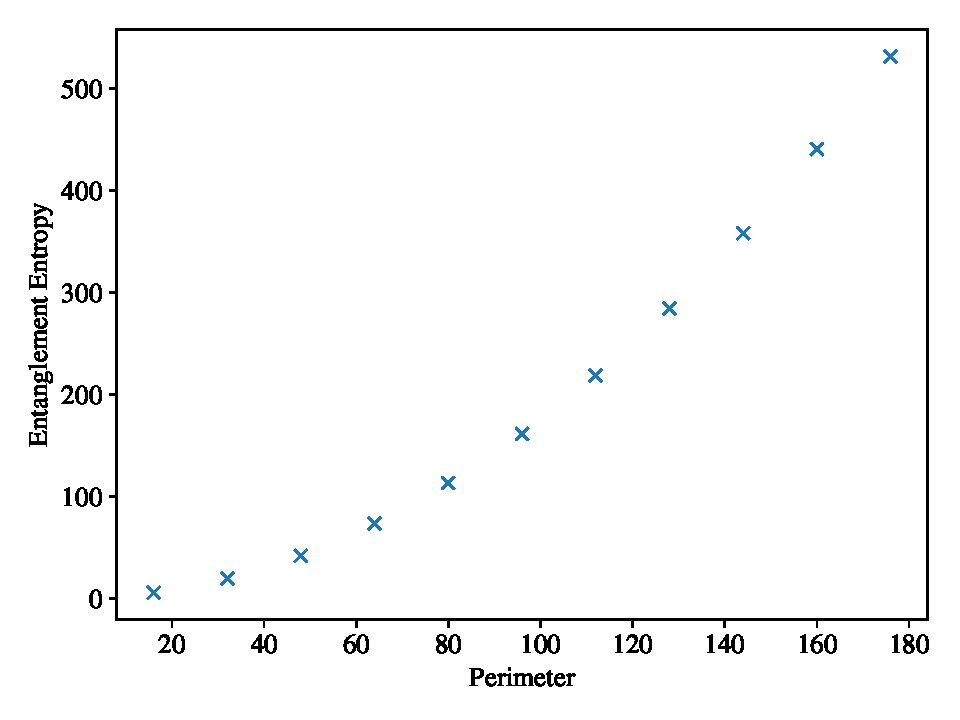
\includegraphics[height=0.15\textheight]{2D_free_fermion_small-region_JustShowData}
  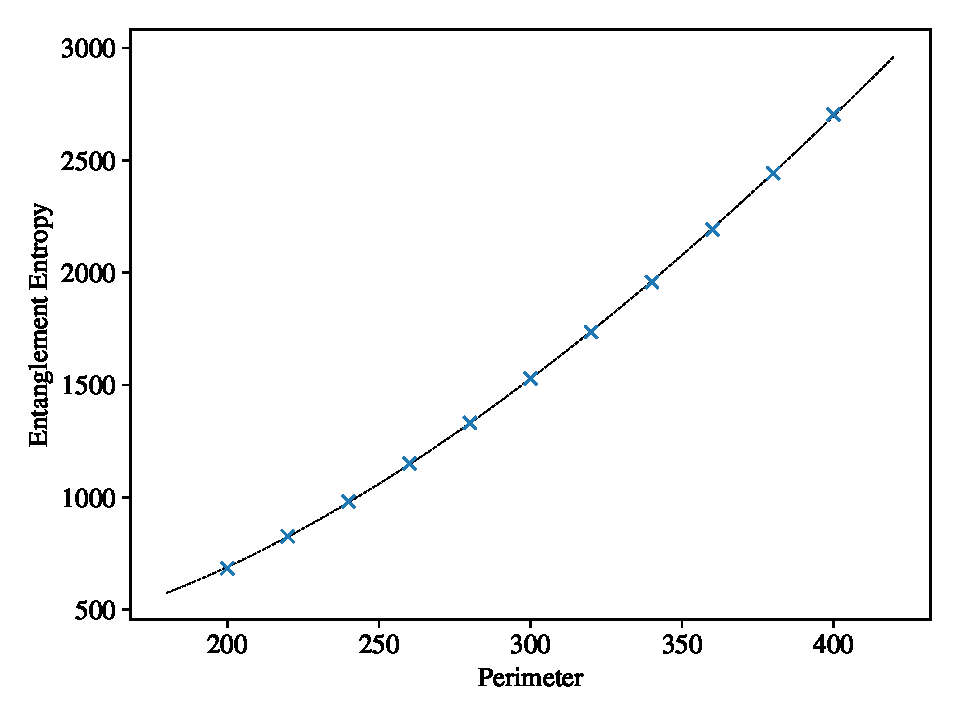
\includegraphics[height=0.15\textheight]{2D_free_fermion_large-region}
  \caption{(a) The entanglement entropy scaling of a one-spacial dimensional free fermion tight binding model with filling fraction $\nu = \anglelr{\hat{n}} = 0.2$, showcasing a perfect $\log L$ behaviour. $L$ is the length of the subregion.  Data points in (b) and (c) are the values of entanglement entropy of a 2D free-fermion tight binding model with filling fraction $\nu = \anglelr{\hat{n}} = 0.2$ computed in square subregions with different sizes. Perimeter of the 2D region stands for the \emph{area}. Data of (c) is fitted with the function $L\ln L$, where $L$ is the perimeter, i.e. the \emph{area} in the context of area-law entanglement.}\label{area-law-free.f}
\end{figure}
\begin{figure}
  \centering
  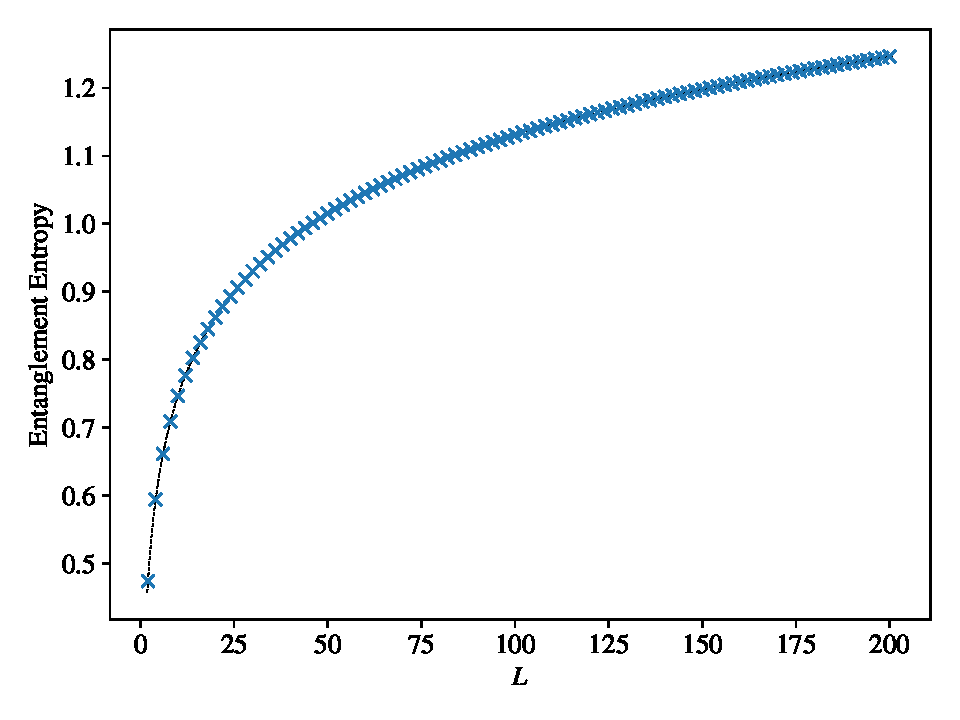
\includegraphics[height=0.2\textheight]{wirelimit_YaoQi_log_fitting}
  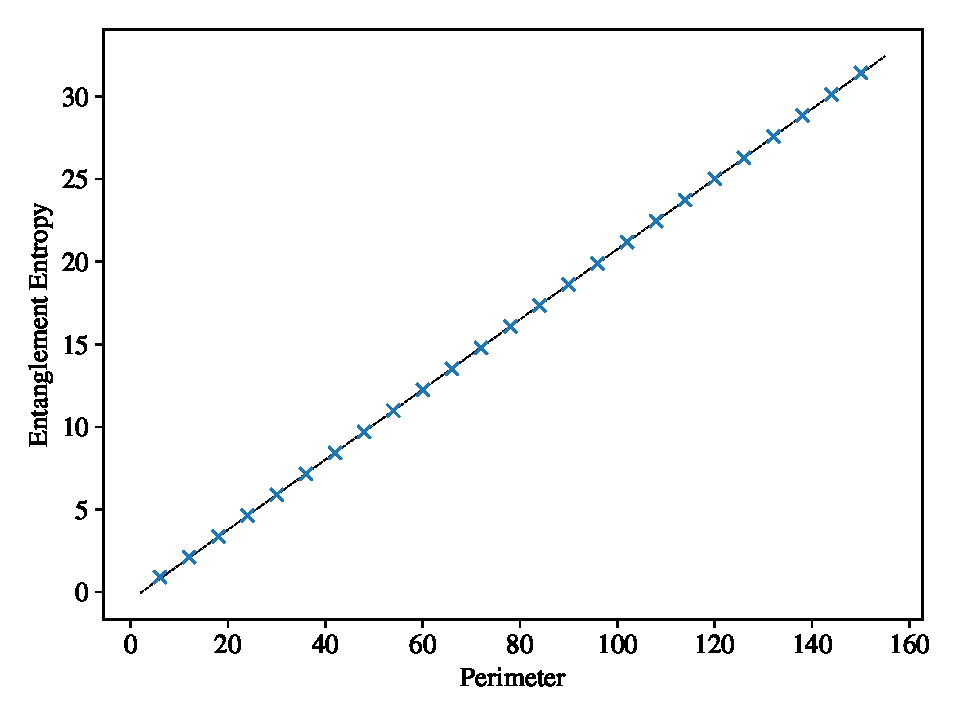
\includegraphics[height=0.2\textheight]{Yao-Qi-2D-ee-square-growth-step_2}
  \caption{(a) The entanglement entropy scaling of the fermion part of the Kitaev model in the wire limit, i.e. $J_x=J_y\gg J_z$. Each data point of the entanglement entropy of a quasi-1D region containing only $x$- and $y$-dimensional bonds, and $L$ is the length of the quasi-1D region. The result showcases a perfect $\log L$ scaling, breaks the area law for one-spacial dimensional systems, and the central charge obtained from the fitting result is $c\approx 0.5$, implying a fermionic CFT. (b) The perfect area-law scaling of the fermion part entanglement entropy of the Kitaev model in the isotropic limit. The entanglement entropy of the fermion part of the Kitaev model is calculated following the theory proposed by Yao and Qi \cite{Qi}.}\label{area-law-Kitaev.f}
\end{figure}
Many theoretical researches \cite{FS-ee_1, FS-ee_2, FS-ee_3, FS-ee_4} have shown that the entanglement entropy scaling of a $d$-spacial dimensional free-fermion system with an open fermi surface is of the form
\[
S\llr{L} \sim L^{d-1}\log L
\]
if Widom's conjecture 
\[
S\llr{L} \sim \frac{L^{d-1}\log L}{\llr{2\pi}^{d-1}}\frac{1}{12}\int_{\de A}\int_{\de \Gamma}\abs{\hat{\bo{n}}_{x}\cdot\hat{\bo{n}}_p}\mrm{d}S_{x}\mrm{d}S_{p}
\]
is true \cite{FS-ee_2, Widom}, where $A$ is the real-space subregion we chose, $\Gamma$ is the region in the momentum space enclosed by the fermi surface, and $\hat{\bo{n}}_{x,p}$ are the normal vectors to $\de A$ and $\de\Gamma$ respectively. Such a result holds when the codimension, defined as the dimension of the momentum space subtracted by the dimension of the fermi surface, is one. For a $d$-spacial dimensional system with an open fermi surface, the codimension is always one because the fermi surface is an $(d-1)$-dimensional object, thus $d-(d-1) = 1$. However, if the free-fermion system has a fermi \emph{point} instead of a open fermi \emph{surface}, then the conjecture doesn't hold anymore for $d$-spacial dimensional system with $d>1$, because now the fermi \emph{point} is a zero-dimensional object, and the codimension is then $d-0=d$, which is not equal to one if $d>1$. However, if $d=1$, then the codimension will still be one, no matter it is the fermi surface or a fermi point. Which explains why the entanglement entropy scaling of a one-spacial dimensional gapless free-fermion system still has the leading term $\log L$ even though there's no well-define open fermi surface. Another explanation comes from (1+1)D conformal field theory (CFT) \cite{CFT_1, CFT_2, CFT_3}, via which physicists have proven that the entanglement entropy scaling of a (1+1)D CFT must have a leading term $\log L$. An one-spacial dimensional system with a gapless dispersion can be described by a (1+1)D CFT, which has nothing to do with the existence of the well-defined open fermi surface. Therefore, an one-spacial dimensional system always has a $\log L$ leading term in the entanglement entropy scaling.

Fig.\ref{area-law-free.f}. shows the entanglement entropy scaling of 1D and 2D free-fermion tight binding model with the Hamiltonian 
\[
H = -t\sum_{\anglelr{ij}}c^{\dagger}_ic_j + \mrm{H.c.}
\]
The fermion correlation function can be computed exactly for 1D. As for 2D cases, we can still obtain an closed form formula by approximating the fermi surface as a circle. The correlation function of a 1D free-fermion system is
\begin{equation}\label{1D-free-correlator.e}
\anglelr{c^\dagger_mc_n} = \nu\frac{\sin\lr{\nu\pi\abs{m-n}}}{\nu\pi\abs{m-n}}
\end{equation}
For 2D, the result is
\begin{equation}\label{2D-free-correlator.e}
  \anglelr{c^\dagger_ic_j} \approx \nu\frac{J_1\lr{\kappa\abs{\bo{x}_i - \bo{x}_j}}}{\kappa\abs{\bo{x}_i - \bo{x}_j}}
\end{equation}
where $\nu = \anglelr{\hat{n}}$ is the filling fraction, and $\kappa \equiv \sqrt{4\pi\nu}$. Equation (\ref{2D-free-correlator.e}) holds only when $\nu\ll 1$. The correlation function of such forms will give the $L^{d-1}\log L$ entanglement entropy scaling. The forms of scaling functions (\ref{1D-free-correlator.e}) and (\ref{2D-free-correlator.e}) arise from the integral
\[
\int_{\abs{k}<k_F}\frac{\mrm{d}^d\bo{k}}{\llr{2\pi}^d}e^{i\bo{k}\cdot \bo{x}}
\]
whose existence relies on the presence of a well-defined open fermi surface.

On the other hand, the correlation functions of the Kitaev model are in a completely different form,
\begin{equation}\label{correlationAB.e}
\begin{aligned}
&\anglelr{c_{\bo{x}A}c_{\bo{x}'B}} = \frac{i}{N/2}\sum_{k}\cos\llrm{k\llr{\bo{x}'-\bo{x}} - \theta_k} \\
&\anglelr{c_{\bo{x}A}c_{\bo{x}'A}} = \anglelr{c_{\bo{x}B}c_{\bo{x}'B}} = 0
\end{aligned}
\end{equation}
The correlation function of the graphene tight-binding model is also in a similar form. Both Kitaev model mean-field theory and the graphene tight-binding model have fermi \emph{points} rather than open fermi surfaces. 

Here I'd like to provide a different physical picture to understand the difference in scaling behaviour between systems with fermi surfaces and fermi points.  Consider a spinless free-fermion system with no sublattice structures having the number of fermions equals the number of lattice sites, the correlation function of elementary excitation $\alpha_{\bo{k}}$ that diagonalizes the Hamiltonian 
\[
H = \sum_{\bo{k}}\epsilon_{\bo{k}}\alpha^\dagger_{\bo{k}}\alpha_{\bo{k}}
\]
is then
\[
\anglelr{\alpha^\dagger_{\bo{k}}\alpha_{\bo{k}'}} = \delta_{\bo{k}\bo{k'}}
\]
Perform the fourier transform, we will also have 
\[
\anglelr{\alpha^\dagger_{i}\alpha_{j}} = \delta_{ij}
\]
And because the elementary excitation is the superposition of original fermions of the model $\alpha_i = \sum_{j}u_{ij}c_j$, where $u_{ij}$ is unitary, we eventually obtain
\[
\anglelr{c^\dagger_i c_j} = \delta_{ij}
\]
If we substitute this result into the correlation matrix, one will obtain that the entanglement entropy is zero. The physical meaning of such a result is that the hopping of the fermions quenches since the lattice is completely filled with fermions such that there's no vacancy at all for those fermions to move toward other places. By end of the day, each fermion just stay at its place and forms an isolated system, hence no entanglement. 

However, the situation will be different if we consider the presence of sublattice structure. Take a half-filled graphene (number of fermions is half of the lattice sites) for example, the Hamiltonian represented in the momentum space is
\[
H = \sum_{\bo{k}}\Psi_{\bo{k}}^\dagger H\llr{\bo{k}}\Psi_{\bo{k}}
\]
where $\Psi_{\bo{k}}\equiv \llr{c_{\bo{k}A}, c_{\bo{k}B}}^T$ and 
\[
H\llr{\bo{k}} = \begin{pmatrix}
                 0 & t(\bo{k}) \\
                 t^*(\bo{k}) & 0 
               \end{pmatrix} \quad,\quad t(\bo{k}) = t\llr{1 + e^{i\bo{k}\cdot\hat{\bo{n}}_1} + e^{i\bo{k}\cdot\hat{\bo{n}}_2}}
\]
Such a Hamiltonian can be diagonalized by fermions $\alpha$ and $\beta$ in the form
\[
H = \sum_{\bo{k}}\abs{t\llr{\bo{k}}}\llr{\alpha^\dagger_\bo{k}\alpha_\bo{k} - \beta^\dagger_\bo{k}\beta_\bo{k}}
\]
The relation between $\alpha,\beta$ and the original fermion $c$ is
\[
\begin{pmatrix}
  \alpha_\bo{k} \\
  \beta_\bo{k} 
\end{pmatrix} = \frac{1}{\sqrt{2}}\begin{pmatrix}
                                    1 & e^{i\theta_\bo{k}} \\
                                    e^{-i\theta_\bo{k}} & -1 
                                  \end{pmatrix}\begin{pmatrix}
                                                 c_{\bo{k}A} \\
                                                 c_{\bo{k}B} 
                                               \end{pmatrix}
\]
Because now the lower band ($\beta$-fermions) is completely filled and the upper band ($\alpha$-fermions) is empty, the correlation function of the ground state, in the Bravais lattice point of view, is 
\[
\begin{aligned}
& \anglelr{\alpha_\bo{x}^\dagger\alpha_{\bo{x}'}} = 0 \\
& \anglelr{\beta_\bo{x}^\dagger\beta_{\bo{x}'}} = \delta_{\bo{x}\bo{x}'} \\
& \anglelr{\alpha_\bo{x}^\dagger\beta_{\bo{x}'}} = 0
\end{aligned}
\]
This seems to imply the quench of hopping of fermions, but it turns out that each site doesn't form an isolated system like in the previous case, because the quench of hopping only happens in the Bravais lattice point of view. The presence of sublattice structure allows fermions to hop in a range of a lattice constant. This is exactly the reason why the entanglement scaling of a system with fermi points still obey the area law even though the dispersion is gapless. Each $\alpha$ and $\beta$ fermion stay at their original position, causing no long-range hopping all over the system, unlike free fermions in a metal that form a non-local metallic bond. So we have no long-range correlation of the form (\ref{2D-free-correlator.e}), hence no contribution to the term $L^{d-1}\log L$ in the entanglement scaling that breaks the area law. However, unlike the previous spinless insulator, the entanglement is not completely zero even though the hopping of elementary excitation quenches. The reason is that the real fermions that describe the physics of the system are $c$-fermions, and they can still hop in a short range of the order of a lattice constant, which form resonant valence bonds and contributes to the short range entanglement, which is exactly the area law we have observed. More specificly, the correlation function of $c$-fermions is
\[
\begin{aligned}
& \anglelr{c^\dagger_{iA}c_{jA}} = \anglelr{c^\dagger_{iB}c_{jB}} = \frac{1}{2}\delta_{ij} \\
& \anglelr{c^\dagger_{iA}c_{jB}} = -\frac{1}{2}\int_{\mrm{BZ}}\frac{\mrm{d}^2\bo{k}}{\llr{2\pi}^2} e^{-i\llrm{\bo{k}\cdot\llr{\bo{x}_i-\bo{x}_j} + \theta_\bo{k}}}
\end{aligned}
\]
we can see that the entanglement is contributed by the fermion hopping between $A$ and $B$ sublattice sites, and which is short-ranged compare to the contribution by the free-fermion with an open-fermi surface (\ref{2D-free-correlator.e}).

One have to notice that such a picture breaks down in one-spacial dimension. The fermions in a one-spacial dimensional gapless free-fermion system can be separated into the \emph{left mode} and the \emph{right mode}, such two modes are independent of each other. Therefore, it doesn't matter whether the system has an open fermi surface or just a fermi point, because the two modes are fully separated and can be seen as two independent chiral gapless systems, in which the fermi surface is not important and won't affect the physics.

\section{Kitaev Model Mean-Field Theory}
The ground state of the Kitaev model can be exactly solved from the following mean-field Hamiltonian
\[
H_{\mrm{MF}} = \sum_{ij}\im J_{\alpha_{ij}}c_ic_j -\abs{K}\sum_{ij}\hat{u}_{ij}
\]
Such a mean-field theory is a free-fermion theory, so the entanglement entropy can be calculated by the correlation matrix technique.

In the Kitaev model, we can define 
\[
\gamma_{i\sigma\aleph} = 
\left\{
\begin{array}{ccc}
  c_i & ; & (\sigma,\aleph)=(0,0) \\
  b^z_i & ; & (\sigma,\aleph)=(0,1) \\
  b^x_i & ; & (\sigma,\aleph)=(1,0) \\
  b^y_i & ; & (\sigma,\aleph)=(1,1) 
\end{array}
\right.
\]
then one can further define the correlation matrix
\[
\Gamma^{(\gamma)}_{i\sigma\aleph,j\sigma'\aleph'} \equiv \anglelr{\gamma_{i\sigma\aleph}\gamma_{j\sigma\aleph'}} \quad;\quad i,j \in A
\]
to calculated the entanglement entropy of the region $A$ by equation (\ref{ee-corr-Maj.e}). Because $\anglelr{b^\mu c}=0=\anglelr{b^\mu b^\nu}$ with different $\mu$ and $\nu$, the correlation matrix can be decoupled into the form of direct sum,
\[
\Gamma^{(\gamma)} = \Gamma^{(c)}\oplus\Gamma^{(b^x)}\oplus\Gamma^{(b^y)}\oplus\Gamma^{(b^z)}
\]
And because $\anglelr{b_i^\mu b_i^\mu} = 1$ and $\anglelr{b_i^\mu b_i^\nu} = \im\delta_{(i-j)\in\mu}\delta^{\mu\nu}$, each $\Gamma^{(b^\mu)}$ can be further block-diagonalized into the following form
\[
\Gamma^{(b^\mu)} = \bigotimes_{\anglelr{ij}\in A\cap\mu} 
\begin{pmatrix}
  1 & i \\
  -i & 1 
\end{pmatrix}_{\anglelr{ij}}
\]
The eigenvalues of each small block are $0$ and $2$, so the entanglement entropy contributed by $b$-Majorana fermions is
\[
-\frac{1}{2}\sum_{\anglelr{ij}}2\ln 2 + \frac{1}{2}N^A\ln 2 = -N^A_b\ln 2 + \frac{1}{2}N^A\ln 2 = \frac{1}{2}\abs{\de A}\ln 2 - N^A\ln 2
\]
in the above we have used the relation
\[
N^A_b = \frac{3}{2}N^A - \frac{1}{2}\abs{\de A}
\]
Apparently, such a result of entanglement entropy is incorrect. \emph{The reason is we didn't include the \textbf{Gutzwiller projection}.} The consequence of this is that the state we considered in the mean-field theory will be \emph{too ordered} in the sense that all of the $\mathbb{Z}_2$ gauge field are equal to 1. 

In this example, we have seen that the correlation matrix technique cannot be used directly in the parton mean-field theory. The mean-field approximation truncates too much entanglement information, such that the entanglement entropy will be underestimated seriously, and eventually leads to an answer that makes no sense.

\section{Entanglement in General Parton Mean-Field Theories}

\begin{thebibliography}{99}
    \bibitem{toeplitz}\href{https://link.springer.com/article/10.1023/B:JOSS.0000037230.37166.42}{B.-Q. Jin and V. E. Korepin, \emph{Quantum Spin Chain, Toeplitz Determinants and the Fisher-Hartwig Conjecture}, J. Stat. Phys. \textbf{116}, 79 (2004)}
    \bibitem{Qi}\href{https://doi.org/10.1103/PhysRevLett.105.080501}{H. Yao and X. L. Qi, \emph{Entanglement Entropy and Entanglement Spectrum of the Kitaev Model}, \emph{Phys. Rev. Lett.} \textbf{105}, 080501 (2010)}
    \bibitem{FS-ee_1}\href{https://doi.org/10.1103/PhysRevLett.105.050502}{Brian Swingle, \emph{Entanglement Entropy and the Fermi Surface}, Phys. Rev. Lett. \textbf{105}, 050502 (2010)}
    \bibitem{FS-ee_2}\href{https://doi.org/10.1103/PhysRevLett.96.100503}{Dimitri Gioev and Israel Klich, \emph{Entanglement Entropy of Fermions in Any Dimension and the Widom Conjecture}, Phys. Rev. Lett. \textbf{96}, 100503 (2006)}
    \bibitem{FS-ee_3}\href{https://doi.org/10.1103/PhysRevA.74.022329}{T. Barthel, M.-C. Chung, and U. Schollw\"ock, \emph{Entanglement scaling in critical two-dimensional fermionic and bosonic systems}, Phys. Rev. A \textbf{74}, 022329 (2006)}
    \bibitem{FS-ee_4}\href{https://doi.org/10.1103/PhysRevB.74.073103}{Weifei Li, Letian Ding, Rong Yu, Tommaso Roscilde, and Stephan Haas, \emph{Scaling behavior of entanglement in two- and three-dimensional free-fermion systems}, Phys. Rev. B \textbf{74}, 073103 (2006)}
    \bibitem{Widom}\href{https://doi.org/10.1007/978-3-0348-5183-1_28}{H. Widom, \emph{On a Class of Integral Operators with Discontinuous Symbol}, In: I. Gohberg (eds) Toeplitz Centennial. Operator Theory: Advances and Applications, vol 4. Birkhäuser, Basel. (1982)}
    \bibitem{CFT_1}\href{https://doi.org/10.1016/0550-3213(94)90402-2}{Christoph Holzhey, Finn Larsen, and Frank Wilczek, \emph{Geometric and renormalized entropy in conformal field theory}, Nucl. Phys. B \textbf{424}, 443 (1994)}
    \bibitem{CFT_2}\href{https://doi.org/10.1088/1742-5468/2004/06/P06002}{Pasquale Calabrese and John Cardy, \emph{Entanglement entropy and quantum field theory}, J. Stat. Mech. P06002 (2004)}
    \bibitem{CFT_3}\href{https://doi.org/10.1088/1751-8113/42/50/504005}{Pasquale Calabrese and John Cardy, \emph{Entanglement entropy and conformal field theory}, J. Phys. A: Math. Theor. \textbf{42} 504005 (2009)}
\end{thebibliography}
\end{document} 